\subsection{Выбор архитектурного подхода и проектирование структуры модулей}

В качестве архитектурного стандарта для разрабатываемой системы выбран
модульный монолит со stateless-характером исполнения. Данный подход позволяет
сохранить целостность приложения и упростить сопровождение системы, при этом
разделив прикладную логику на изолированные функциональные блоки с явными
границами ответственности.

Выбор именно такого архитектурного решения обусловлен следующими факторами:
\begin{enumerate}
    \item тесная связанность процессов индексации, хранения и выдачи данных;
    \item необходимость общей транзакционной модели работы с хранилищем;
    \item сравнительно ограниченный масштаб проекта по сравнению с распределенной
    микросервисной архитектурой;
    \item требование к сохранению stateless-характера приложения при хранении
    критического состояния во внешней базе данных;
    \item потребность в дальнейшем расширении за счет модулей, а не за счет
    немедленного дробления на независимые сервисы.
\end{enumerate}

С инженерной точки зрения модульный монолит в рассматриваемой задаче
представляет компромисс между целостностью доменной логики и требованием к
локализации ответственности внутри приложения. Критическое состояние при этом
хранится во внешней базе данных, что обеспечивает воспроизводимость запуска и
возможность повторного развертывания экземпляра без сохранения локального
сессионного состояния.

Компонентная структура проектируемой системы приведена на
рисунке~\ref{fig:component-c4-design}. Диаграмма отражает взаимодействие
основных модулей серверной части с внешними системами и прикладными клиентами.

\begin{figure}
  \centering
  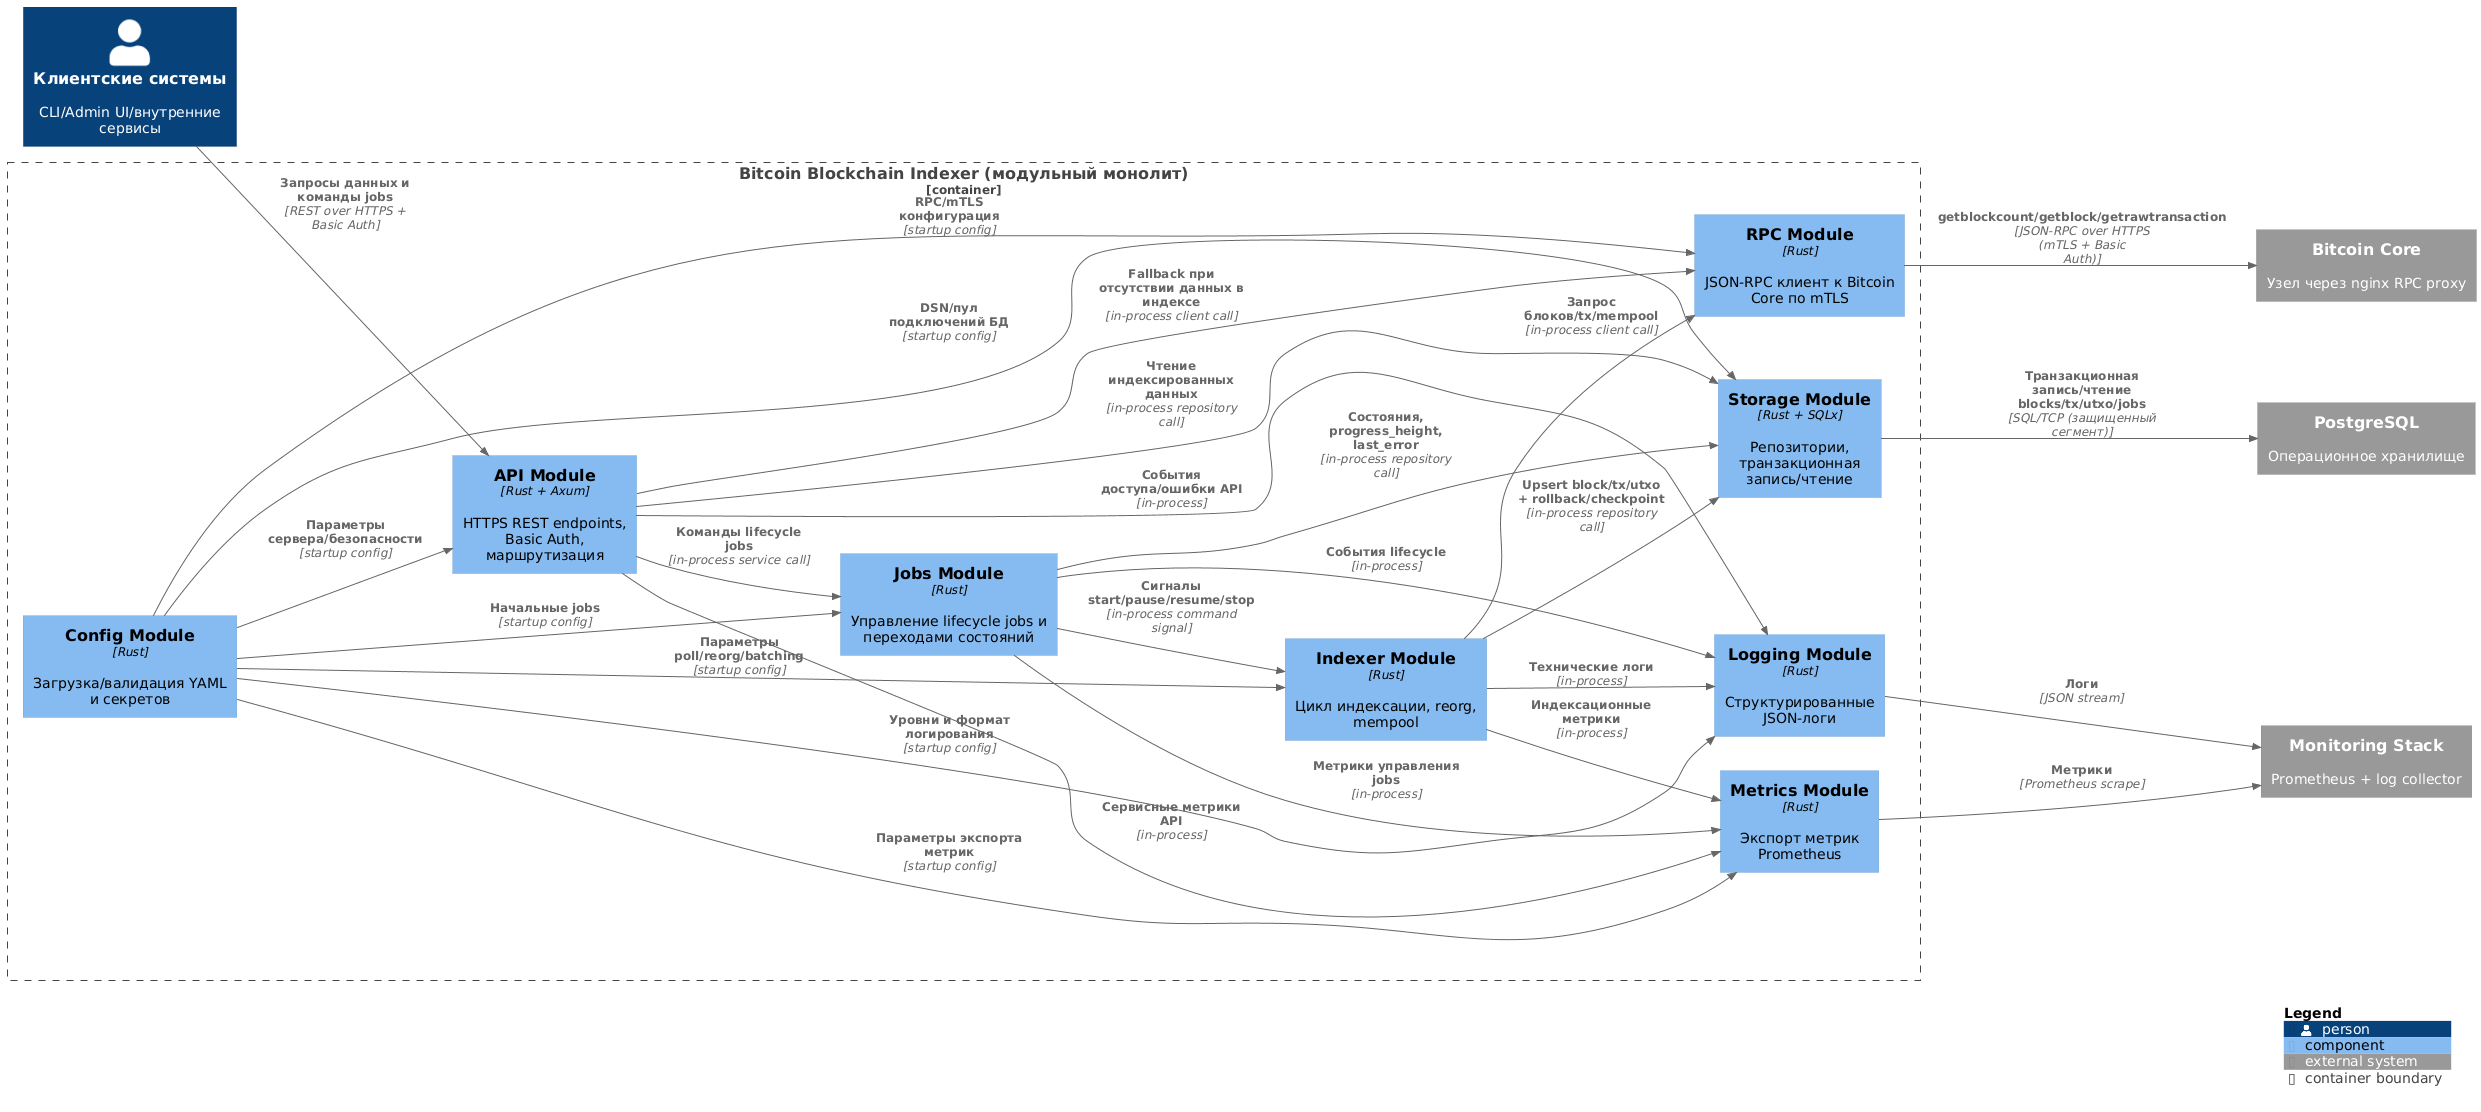
\includegraphics[width=0.9\linewidth]{../report/c4/C4_Component_Architecture.png}
  \caption{Компонентная архитектура системы индексации ончейн-данных}
  \label{fig:component-c4-design}
\end{figure}

В проектируемой системе выделены следующие основные модули:
\begin{itemize}
    \item \texttt{config} --- загрузка и валидация конфигурации, разрешение секретов;
    \item \texttt{api} --- предоставление HTTP API и маршрутизация запросов;
    \item \texttt{indexer} --- получение и сохранение подтвержденных блоков и транзакций;
    \item \texttt{jobs} --- управление заданиями индексирования и их жизненным циклом;
    \item \texttt{mempool} --- синхронизация неподтвержденных транзакций;
    \item \texttt{data} --- прикладные выборки из хранилища;
    \item \texttt{nodes} --- мониторинг состояния подключенных узлов;
    \item \texttt{storage} --- репозитории и транзакционная работа с PostgreSQL.
\end{itemize}

Такое разбиение позволяет локализовать ответственность каждого модуля,
обеспечить независимое развитие отдельных частей системы и минимизировать
влияние локальных изменений на общую архитектуру. Тем самым структура модулей
не только отражает текущую реализацию, но и служит средством обеспечения
расширяемости и сопровождаемости программного комплекса.
